% !TeX root = Bericht.tex
% !TeX spellcheck = en_US
\section{Results}
In order to determine the half-wave-voltage, the intensity was measured by the photodiode, with an inserted triangle voltage with amplitude \SI{3}{V} and a frequency of \SI{30}{Hz}. For the evaluation, the range from minimum to maximum voltage was taken. This interval of voltage is plotted against the intensity. A fit based on \autoref{transmittance} is done, as the intensity is proportional to the transmittance. There were several measurements made to gather statistics, in \autoref{voltage_intensity_pi}, one example of a fit is shown. From this measurement, we get $V_{\pi,FG} = 2.24(1) \unit{V}$ for the measurements including the $\lambda/2$-waveplate. The voltage given here refers to the voltage that has to be inserted at the function generator. At the EOM, the voltage is actually 100 times bigger, as an amplifier is used. The uncertainty of the amplifier is neglected here, as it is estimated to be very small in contrast to the determined value of the voltage. As an average value (without $\lambda/2$-waveplate) we get 
$$V_{\mathrm{\pi, mean}}=\SI{451.9(5)}{V}.$$ 
This value is already multiplied by 100, as the amplifier outputs the monitor signal at a reduced level. The uncertainty here is calculated as the standard deviation of the values for $V_{\pi}$.  Using this value and \autoref{volt_pi_relation}, the material based factor $r_{13}n_O^3$ can be determined as 
$$r_{13}n_O^3=\SI{103(6)}{pm/V}.$$
When we use the value of $n_O$ from the script, which is given as 2.2865, we get $$r_{13}=\SI{8.9(5)}{pm/V}. $$

\begin{figure}[h].
	\centering
	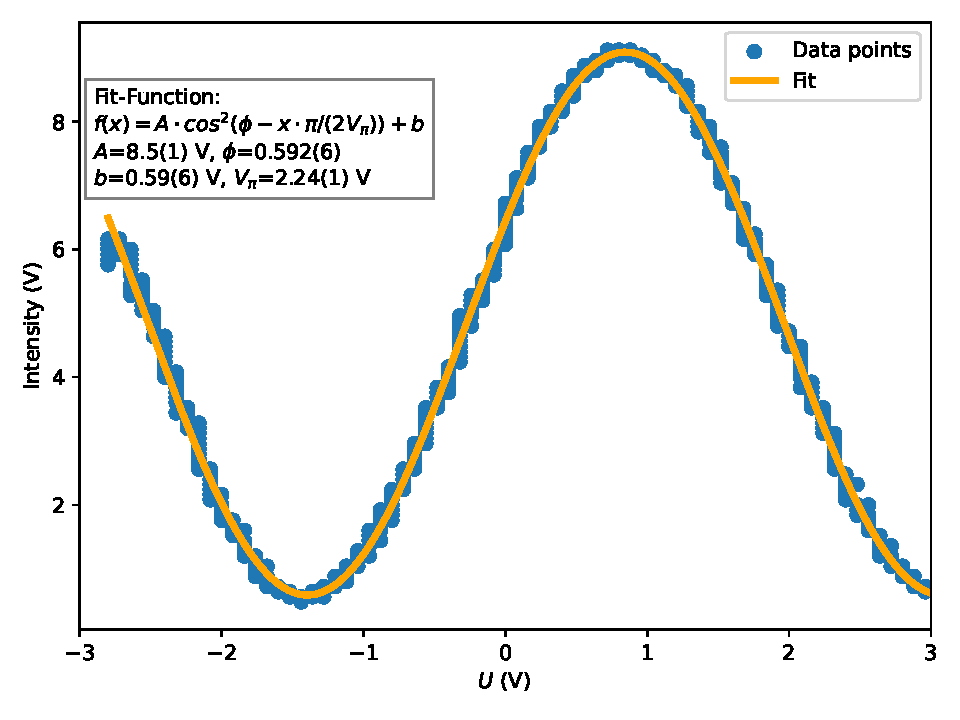
\includegraphics[width=0.8\textwidth]{voltage_intensity_pi}
	\caption{The measured voltage of the photodiode is shown, depending on the input voltage $U$. A fit was done to determine the half wave voltage, the function and parameters are given in the plot.In this plot, only one of several measurements is shown as an example for a measurement including the $\lambda/2$-waveplate, in the later analysis, the results from many measurements are averaged.}
	\label{voltage_intensity_pi}
\end{figure}

When averaging over all of these measurements with the $\lambda/2$-waveplate , we get
$$V_{\mathrm{\pi, mean, waveplate}}=\SI{223.6(3)}{V}.$$
Which yields to
$$r_{33}n_e^3=\SI{208(12)}{pm/V}$$
and width the value for $n_e$ , given in the script as 2.2022 \autocite{eom}, we get a value of $$r_{33}=\SI{19.4(1.1)}{pm/V}.$$




%The voltage given here refers to the voltage that has to be inserted at the function generator. At the EOM, the voltage is actually 100 times bigger, as an amplifier is used. 
%When analysing the measurements without the $\lambda/2$-waveplate, we get a mean value of 
%$$V_{\mathrm{\pi, mean, no waveplate}}=\SI{1.236(3)}{V}.$$
%Using this value and \autoref{volt_pi_relation}, the material based factor $r_{33}n_e^3$ can be determined as $$r_{33}n_e^3=\SI{208(12)}{pm/V}. $$
%The absolute value for $n_e$ is given in the script as 2.2022 \cite{eom}, so we get a value of $$r_{33}=\SI{19.4(1.1)}{pm/V}.$$


In the next step, the bandwidth of the first setup was determined qualitatively. The bandwidth is defined as the frequency, at which the interference contrast decreases clearly, compared to the contrast at low frequency. In our case, we use the frequency, at which the contrast is half the contrast at the lowest measured frequency, which was \SI{30}{Hz}. At \SI{30}{Hz}, the contrast is 0.87(2), so we are looking for the frequency with a contrast of 0.434(8). To estimate this quantity, a exponential function is fitted to the data points, which are the contrast at different frequencies. The reason for the choice of an exponential is, that it describes the behaviour in the relevant measured range well. The data as well as the fit function with parameters are shown in \autoref{contrast_frequency_bandwith_plot}. Using the aforementioned definition of bandwidth and the fit parameters, we are getting a bandwith of \SI{425(10)}{Hz}. 

\begin{figure}[H]
	\centering
	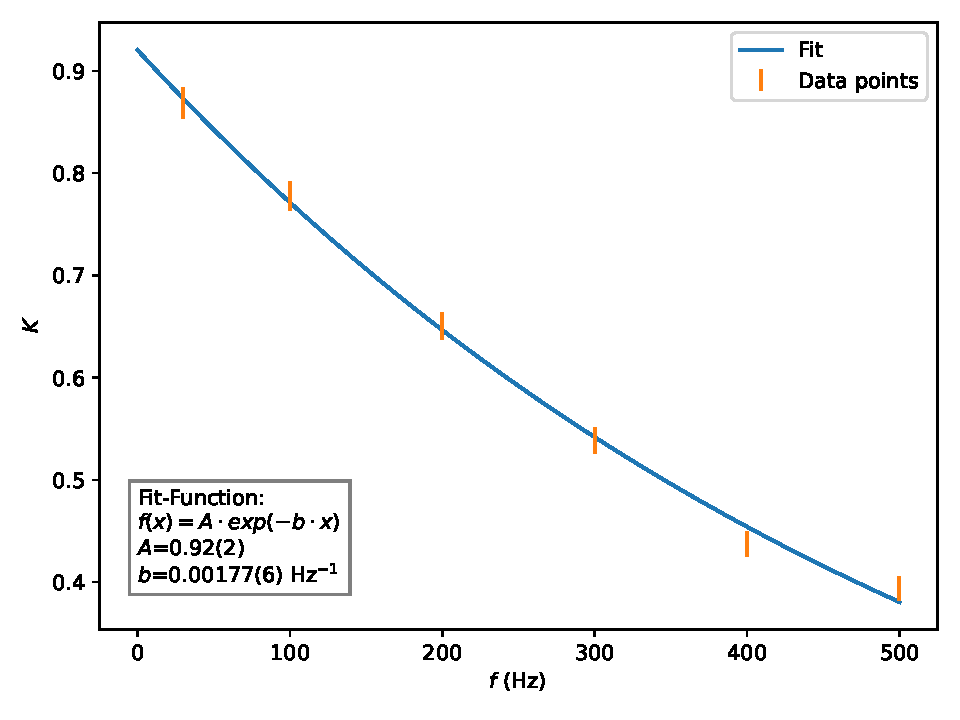
\includegraphics[width=0.7\textwidth]{contrast_frequency_plot}
	\caption{The measured interference contrast is shown dependent on the input frequency $f$. Additionally, an exponential fit is shown, parameters and function are shown in the graph. }
	\label{contrast_frequency_bandwith_plot}
\end{figure}
\begin{figure}[H]
	\centering
	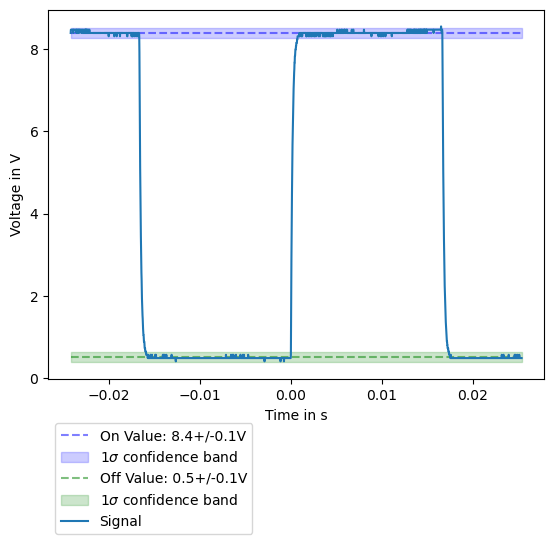
\includegraphics[width=0.7\linewidth]{BildSwitch}
	\caption{The EOM's behaviour as an optical switch can be seen. The average on voltage and off voltage are also shown. To determine these, the rising and falling edges were first determined. Then the system was given a settling time of 0.0003 s. The mean value up to the next edge was then determined. In each case, the standard deviation serves as uncertainty. This is visualized with a $1\sigma$ confidence band.}
	\label{fig:Switch}
\end{figure}




For the second set-up, we implemented an optical switch at the same frequency as before, but with a square-wave signal. However, it is first necessary to determine the value of $V_{\pi,2}$. This is done according to the same procedure as for the data from the first setup. The value of 
$$V_{\pi,2}=\SI{152.16(7)}{V}$$
was determined. Thereafter, the offset voltage and the amplitude of the square wave signal were manually adjusted until the maximum on/off ratio was achieved. This can be seen in  \autoref{fig:Switch}. We repeated the measurement once and determined an on/off-ratio of $V_\mathrm{ON}/V_\mathrm{OFF}=17(4) $ and $V_\mathrm{ON}/V_\mathrm{OFF}=18(5)$. To determine the $V_\mathrm{ON}$ and $V_\mathrm{Off}$, we first searched for the Flank and then calculated the mean value up to the next Flank after a transient phase of 0.0003 s. We used the standard deviation as the uncertainty. The value for the transient phase was not chosen at random; it was approximately 2 times the half-life for the reaction of the system. We will discuss this further later.


To get an idea of the response time of the system, a falling edge was observed for a square wave signal. With the original setup we obtained a half-life of $1.3\cdot 10^{-4} \unit{s}$. To bridge the internal resistance of the oscilloscope, a $50\:\unit{\ohm}$ resistor was connected in parallel. Although the measured signal is much smaller than in the original setup, a half-life of $1.9\cdot 10^{-6} \unit {s}$ can be obtained. As these are qualitative and not quantitative values, no error calculation was made. For better comparison in the graph, the amplitudes have been normalised to $\pm 1$. The final slope analyses can be seen in \autoref{fig:Flankenverhalten}. It can be seen that the half-lives differ by 2 decimal points.

\begin{figure}[H]
	\centering
	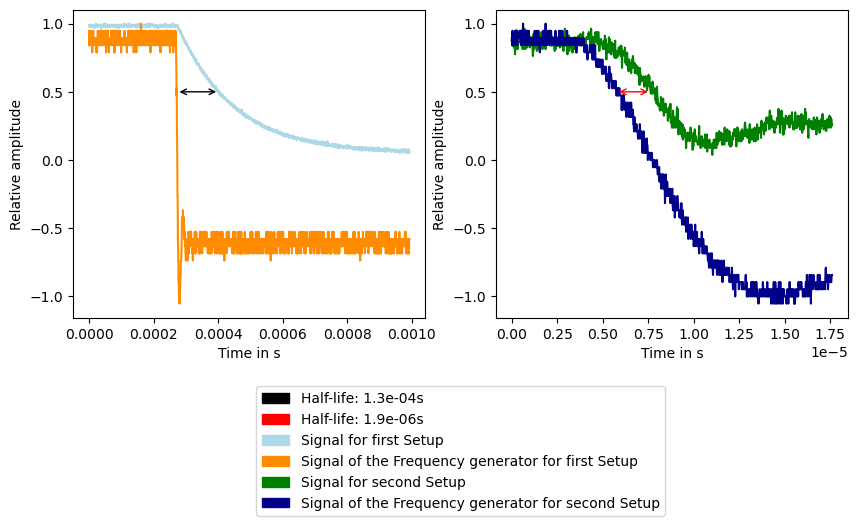
\includegraphics[width=\linewidth]{BildReaktionszeit}
	\caption{The response behaviour of the system can be seen. In the left picture the setup was made as befor and in the right picture a $50 \unit{\ohm}$ resistor was connected parallel to the oscilloscope to minimise the input resistance. The signals have been normalised to their maximum at $\pm 1$. The signal from the frequency generator, the recorded signal from the laser diode and the half-life can be seen.}
	\label{fig:Flankenverhalten}
\end{figure}






